\section{Background}
\subsection{SIMD}

SIMD stands for Single Instruction Multiple Data.  This is a parallelisation
technique where the program issues a single instruction such as an ADD to the
CPU core which is then applied to multiple pieces of data at once.  By doing
this any workflow that can be re-written to use the same series of instructions
on a set of data can be sped up a lot.  The most common example of this type of
parallelism is in Graphics Processing Units (GPUs)
\cite{Fatahalian:2008:CLG:1400181.1400197}, these are required to perform the
same transformation to millions of polygons simultaneously and so by utilising
an SIMD architecture consisting of literally hundreds of parallel units they
obtain massive speed ups.

The basic implementation of an SIMD processor is to 

\subsection{Leros}
In order to avoid carrying out redundant work, a decision was made to utilise an
existing solution as a base development. The advantages were twofold; not only
did it allowed for much faster development, but had already been tested by many
people. Opencores\footnote{\url{http://www.opencores.com}}
is a large open-source hardware community, well-known for its collection of hardware solutions for
FPGAs and ASICs, in both VHDL and Verilog. Our requirements called for a VHDL
microcontroller, of which there were many to choose from. Other criteria included
simplicity of code, small code size, and a RISC architecture. One project stood out
after applying these critera, named the \emph{Leros} microcontroller after the
Greek Island Leros \cite{schoeberlleros}.  The Leros MCU is a 16-bit
processor optimized for FPGAs \cite{schoeberlleros}, and was selected for use in this
project.

 It is a stable
project and can even be programmed in a restricted subset of Java. It is licenced
under the permissive BSD licence and has been tested under the Xilinx toolchain.
Leros' architecture is a pipelined 16-bit accumulator processor\ref{schoeberlleros},
with instructions executed in a single cycle.

The accumulator architecture made Leros an attractive option for this project.

\begin{figure*}[h]
\center
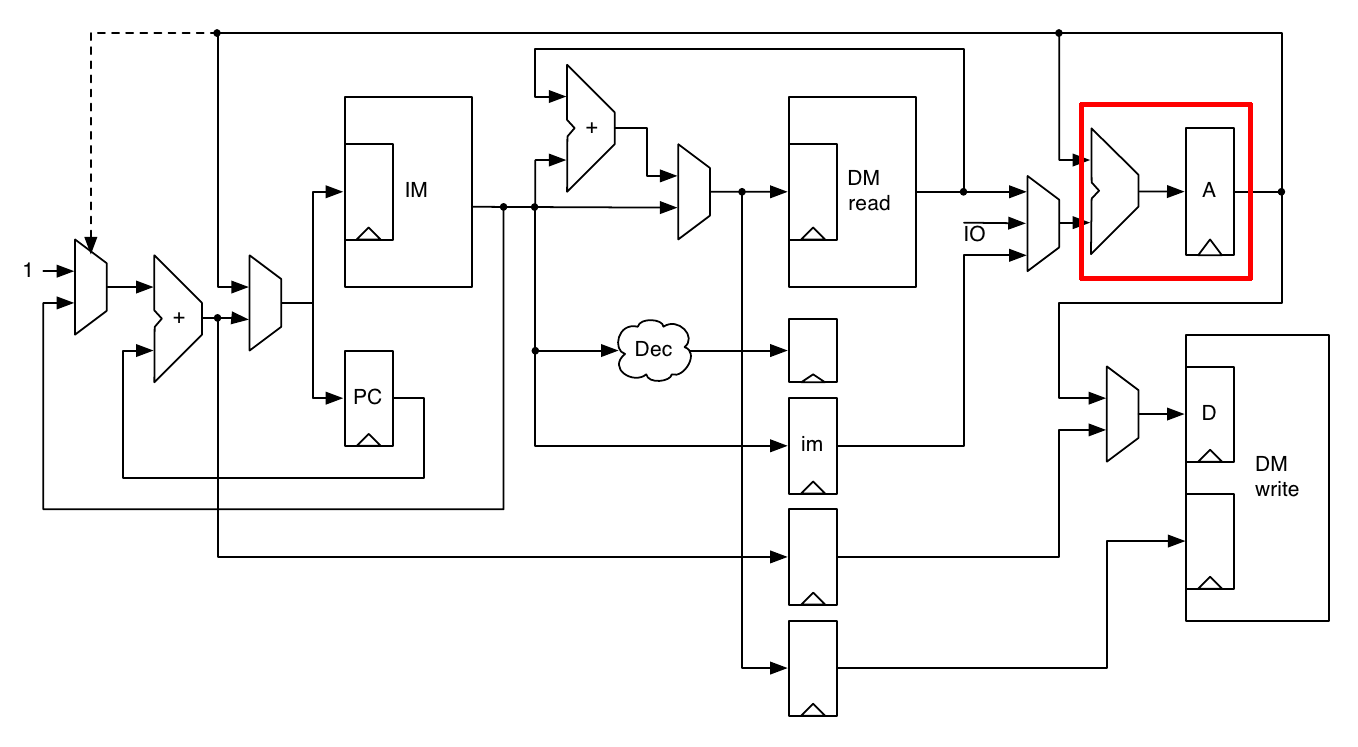
\includegraphics[width=0.9\textwidth]{images/leros-system}
\caption{Leros pipeline. The section of the design to be multiplied has been
highlighted in red. Original image from \cite{schoeberlleros}.
}
\label{fig:leros-system}
\end{figure*}
